\section{Overview}
\label{sec:overview}

\begin{figure*}[t]
\centering
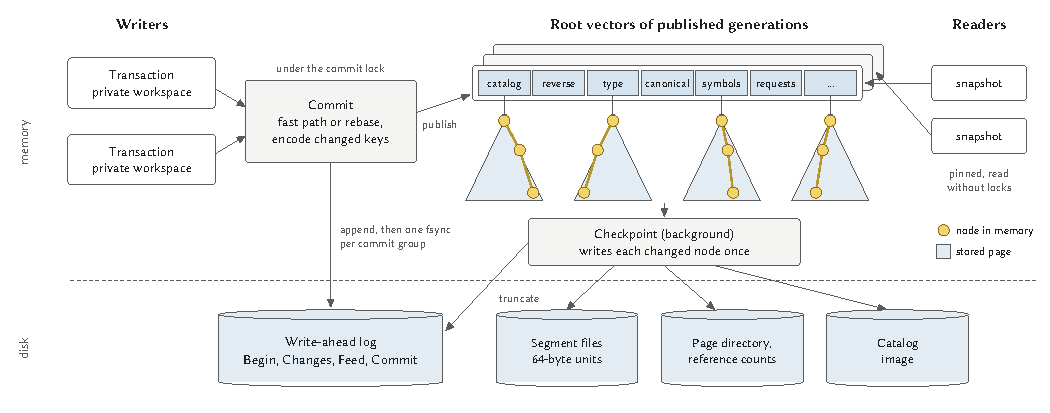
\includegraphics[width=\textwidth]{figures/overview}
\caption{Engine overview. A commit appends the keys it changed to the write-ahead log and publishes a new root vector whose changed nodes (yellow) are still in memory, on top of stored pages (blue). Readers pin a generation and read it without locks. A background checkpoint writes the changed nodes, syncs them, publishes a catalog image and truncates the log.}
\label{fig:overview}
\end{figure*}

\Cref{fig:overview} shows the main parts of the engine. The state of the database at one point in time is a \emph{generation}: a small immutable object that holds, for each branch, a \emph{root vector} that maps a slot number to the root of a tree. The engine defines seven slots: the \emph{catalog} of atoms, the reverse incidence index, an index from type to atoms, an index of canonical keys, two symbol tables for role names, and a table of request ids that makes retried commits idempotent. The database layer adds its own slots for schemas, properties, property indexes and the like. Slots are either primary, written by transactions, or derived, maintained from the primary slots inside the same transaction by \emph{derivations}. The reverse incidence index is derived from the catalog.

All trees are copy-on-write. A transaction works on a private copy of the root vector, and its writes copy the paths they change. A commit publishes a new generation that shares every unchanged subtree with its predecessor. Readers pin a generation and never take a lock. Writers serialise only on a short section of the commit that assigns the generation number and appends to the log, and commits that reach the log while an earlier batch is being synced share one fsync.

The tree nodes a commit creates are not written at commit time. The commit logs the keys it changed and publishes nodes that are still in memory; a background checkpoint later writes them to pages. Pages are packed into append-only segment files and found through a page directory, so that compaction can move them without changing any tree. The rest of the paper follows this structure: trees and the on-disk layout (\cref{sec:layout}), commits, checkpoints and recovery (\cref{sec:transactions}), and reclaiming space (\cref{sec:space}).
